\section{Introduction}

A mixture-of-experts (MoE) language model routes each token to a subset of
its feed-forward experts. The resulting sequence of expert selections
provides an internal view of how computation changes while the model
solves a problem. A useful account must distinguish three questions:
which reasoning states routing describes, which changes routing predicts,
and whether changing that routing improves the solution or its cost.
The answer to one question does not determine the others.

We examine seven checkpoints: GPT-OSS-20B, Nemotron-3.5-Lightning-30B-A3B,
Qwen3.5-35B-A3B, Qwen3.6-35B-A3B, Gemma-4-26B-A4B,
GLM-4.7-Flash and Qwen3-30B-A3B. The preserved corpus contains benchmark
answers, routing captures and reasoning labels. Its common analysis
supports model comparisons without equating expert indices or router
score scales across architectures. Problem families define independent
units; sentences, tokens and repeated answers supply measurements within
those units.

Our main contribution has two seven-model results. First, routing adds
held-out information about reasoning labels beyond the specified text
baseline. Second, a training-only comparison of expert keep-sets shows
that balancing reasoning classes improves minimum held-out coverage in
five models, while pooled labelled frequency performs better in two.
A separate two-model next-class analysis tests predictive information
before the destination sentence. Together these results distinguish
information about reasoning episodes from a useful rule for allocating
experts. The deployment question remains whether a chosen keep-set can
reduce resident expert memory while preserving answer accuracy; the
saved-route analyses do not answer it.

The main text reports the comparable analysis first. Appendices preserve
the historical annotation, probing, three-model correlations, interventions,
current verification audit and full figure atlases. These studies retain
their own populations and measurement rules. They are evidence for
particular parts of the workflow, rather than repeated estimates of one
common effect.

\section{Reasoning Labels, Model Contracts and Benchmarks}
\label{sec:analysis-design}

\subsection{Reasoning labels and related approaches}
The episode vocabulary is Read, Analyze, Explore, Plan, Implement, Verify
and Monitor. The annotation and external probing studies build on the
released SAT-response annotations of \citet{li2025schoenfeld}. The prompt
selection procedure uses GEPA \citep{agrawal2026gepa}; the layerwise
prospective probing design adapts \citet{sun2026trajectories}. These are
labels assigned to text, not independently established modules inside a
model. When a classifier predicts such a label from routing, the supported
claim concerns the information in routing about that label.

The benchmark selection and repeat counts adapt the
mathematical evaluation suite used by \citet{liu2025spiral}.
Expert intervention is related to the (de)activation approach of
\citet{fayyaz2025steermoe}, while our historical policies retain their own
selection estimator, implementations and evaluation populations. We do
not treat those policies as a complete replication of that method.

Expert pruning already has dedicated methods. EAC-MoE combines router
calibration for quantization with pruning based on selection frequency
\citep{chen2025eac}. REAP instead uses routing weights together with
expert-output magnitudes in its pruning criterion \citep{lasby2026reap}.
Counterfactual routing analysis holds model parameters fixed and compares
native routes with alternatives using equal computation
\citep{yoon2026misrouted}. These works make frequency, activation-sensitive
selection and alternative-route evaluation relevant comparisons. Our
comparison adds reasoning-class balance to a controlled seven-model
selection analysis using training families only. A new pruning
claim requires a controlled comparison with relevant pruning methods.

\subsection{A model-specific routing contract}
Let $S_{\ell,t}$ be the selected expert set at routed layer $\ell$ and token
position $t$, and let $k_\ell=|S_{\ell,t}|$ be its native size. Every expert
identity includes checkpoint, layer and local index. A capture binds its
token ownership, score space, selection rule and any shared-expert path.
This matters for architectures with sigmoid scores, correction biases,
grouped selection or learned scaling; a common raw-score manipulation need
not implement a common action.

\begin{table}[t]
\centering\small
\begin{tabular}{lrrr}
\toprule
Model & Routed layers & Expert pool & Native $k$ \\
\midrule
GPT-OSS & 24 & 32 & 4 \\
Nemotron & 23 & 128 & 6 \\
Qwen3.5 & 40 & 256 & 8 \\
Qwen3.6 & 40 & 256 & 8 \\
Gemma & 30 & 128 & 8 \\
GLM & 46 & 64 & 4 \\
Qwen3-30B & 48 & 128 & 8 \\
\bottomrule
\end{tabular}
\caption{Captured routed-layer and selection contracts for the seven
checkpoints. Routed layers exclude dense blocks; expert pools and local
indices do not align across models. Exact checkpoints and quantization
belong to the source manifest.}
\label{tab:model-routing-contracts}
\end{table}

\subsection{Benchmark populations and answer scoring}
The six benchmarks are AIME24, AIME25, AMC23, MATH-500, OlympiadBench and
Minerva. The complete native benchmark corpus contains 4,647 attempts per
model over 1,547 source questions: 32 attempts per AIME24/AIME25/AMC23
question and one on the other benchmarks. The routing analyses use their
own captured subsets. In particular, the latest seven-model observational
A corpus contains 1,547 attempts per model, one per source question; the
repeated B cohort contains 895 attempts but only 51 distinct questions in
the cross-model union. The historical benchmark run likewise contains
4,647 attempts for each of all seven models under its original deployment
contract; the older report sections analyzed three-model subsets of that
run. These populations must not be pooled into a new independent sample.

% Generated by report/model-analysis-review-20261008/build_inventory.py; existing scores only.
\begin{table}[t]
\centering
\small
\caption{Saved seven-model card-profile mathematical accuracy (\%). Each model has 4,647 assigned attempts on the same 1,547 problems (32,529 attempts in total). AIME24/25 and AMC23 use 32 samples per problem; the other datasets use one. Entries are adjudicated accuracy among scored attempts. $U$ counts unresolved attempts per model, retained separately. These checkpoints use different native decoding profiles and output limits; this table is a benchmark description, not an equal-budget architecture comparison.}
\label{tab:seven-model-saved-math}
\resizebox{\linewidth}{!}{%
\begin{tabular}{lrrrrrrr}
\toprule
Model & AIME24 & AIME25 & AMC23 & MATH500 & Minerva & Olympiad & $U$ \\
Problems & 30 & 30 & 40 & 500 & 272 & 675 & \\
\midrule
GPT-OSS & 78.7 & 76.0 & 97.3 & 97.0 & 69.1 & 83.2 & 11 \\
Nemotron & 87.8 & 87.2 & 99.8 & 98.8 & 73.5 & 88.6 & 0 \\
Qwen3.5 & 94.0 & 88.3 & 100.0 & 99.4 & 73.4 & 92.3 & 1 \\
Qwen3.6 & 94.8 & 89.7 & 100.0 & 99.6 & 74.8 & 92.0 & 2 \\
Gemma & 90.8 & 86.8 & 99.7 & 99.0 & 75.6 & 90.8 & 15 \\
GLM & 93.2 & 89.6 & 99.4 & 98.4 & 73.1 & 90.5 & 2 \\
Qwen3-30B & 80.2 & 71.1 & 97.7 & 98.0 & 75.6 & 84.6 & 2 \\
\bottomrule
\end{tabular}}
\par\smallskip\parbox{\linewidth}{\footnotesize The source inventory retains strict scores, all denominators, completion-token costs, caps, and the original question-bootstrap 95\% intervals. Unresolved outcomes total 33; repeated samples are not independent questions. The historical 32k campaign is a separate 32,529-attempt population.}
\end{table}


Accuracy tables retain their source scorer and missing-answer rules.
Token-limit completions and scoring failures remain visible; a comparison
on scorable answers is not accuracy over all assigned requests. Historical
intervention comparisons were separately rescored under a common
answer-equivalence rule, so their values do not overwrite observational
labels. Mathematical benchmark scores describe the workload and anchor
utility evaluation; high native accuracy does not establish the effect of
a proposed routing policy.

\section{Routing Information About Reasoning States}
\label{sec:routing-information}

The CLEAN present-class analysis covers 522 questions and 509 problem
families for each checkpoint. It compares routing-augmented prediction
with a retrospective baseline that already observes the annotation
reader's text context. Families are held together during fitting and
assessment. The saved seven-comparison simultaneous intervals for the
loss difference exclude zero in all seven models
(Figure~\ref{fig:routing-readout}). Lower cross-entropy favors routing.
Separately reported lexical-null excess intervals also exclude zero under
their saved procedure.

The readout uses multinomial ridge classification with five outer and
three inner duplicate-family folds. The baseline includes token-identity
features, position and sentence length, together with the original
previous, current and next sentence text available to the annotation
reader; a missing sentence stays missing. Routing adds top-1 expert
histograms reduced to 64 components, depth-path surprise and temporal
persistence. Learned transforms and regularization are fitted within
training folds. Questions receive equal total weight. The saved
uncertainty resamples whole duplicate families 5,000 times, retaining that
question-weighted estimand. Five lexical-null draws permute token routing
paths within token-identity and absolute-position strata and repeat the
same fitting procedure. These controls test incremental information
about the assigned label, not an online recognition policy.

\begin{figure}[t]
\centering
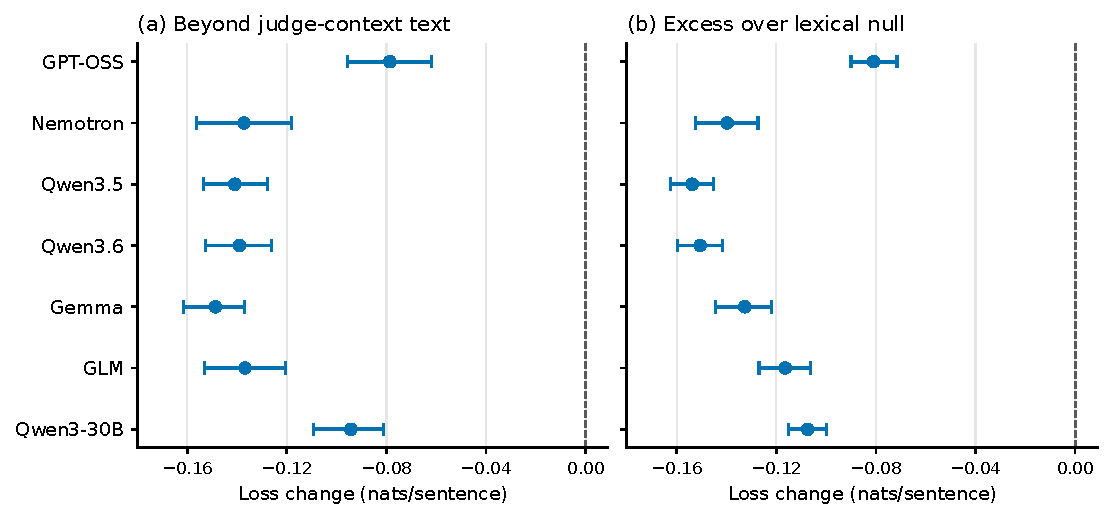
\includegraphics[width=\linewidth]{generated/best_results_20261009/routing_readout.pdf}
\caption{Held-out present-class readout on the common 522-question,
509-family population. (a) Routing-augmented minus retrospective
judge-context loss. (b) Routing-augmented minus the mean lexical-null loss.
Negative values favor routing. Bars copy the original model-specific
seven-comparison 95\% intervals; they are not a joint simultaneous test
across all models and both panels. Questions receive equal weight;
sentences within questions are repeated measurements. Exact values are
in Appendix~\ref{sec:saved-data-supplement}.}
\label{fig:routing-readout}
\end{figure}

This common direction grounds further reasoning-state and expert
analyses: expert allocation contains information beyond the declared text
baseline. The sizes of the gains are conditional on each model's generated
text and label coverage. Comparing the rows does not by itself identify a
more interpretable model or a more effective intervention layer.

An independent part of the evidence concerns prospective hidden-state
probes on externally supplied SAT responses. Five response-disjoint folds
and inner-validation layer selection yield macro-AUROC 0.852
$[0.838,0.868]$ for Qwen3.5, 0.780 $[0.761,0.797]$ for GPT-OSS and 0.788
$[0.772,0.805]$ for Gemma. Each exceeds the corresponding prefix-position
baseline. These intervals resample 38 responses conditional on the saved
folds and fits. The result supports held-out-response information on the
external corpus; it does not establish a deployable detector on each
model's own generations. The complete probe analysis remains in the
appendix.

\section{Next-Class Prediction}
\label{sec:temporal-experts}

An adjacent-state prediction uses the original sentence order. Missing
labels and sentence gaps break adjacency. Descriptive transition matrices
for all seven models remain in Appendix~\ref{sec:saved-transitions}; they
describe observed labelled adjacencies rather than complete trajectories.

The stricter historical next-class analysis asks whether routing observed
before the destination adds to past text/history and a training-only
estimate of the current class. GPT-OSS improves log loss by $0.02073$
nats per pair on 10,209 adjacent pairs from 509 questions; Qwen3.6 improves
it by $0.05570$ on 2,492 pairs from 494 questions. The candidate-minus-baseline
intervals are respectively $[-0.02548,-0.01601]$ and
$[-0.06944,-0.04154]$ under the saved six-comparison correction.
Contained-window sensitivities retain the direction, with substantially
smaller support: 797 pairs for GPT-OSS and 213 for Qwen3.6
(Figure~\ref{fig:next-class}).

\begin{figure}[t]
\centering
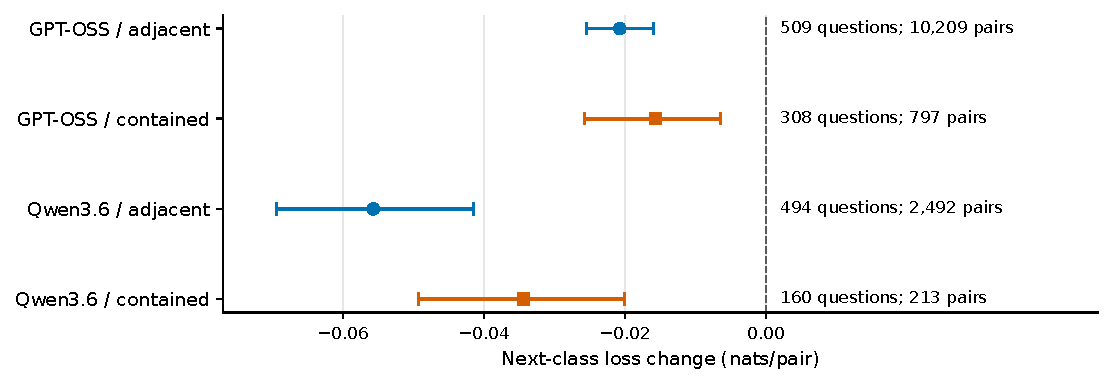
\includegraphics[width=\linewidth]{generated/best_results_20261009/next_class.pdf}
\caption{Next-class loss changes for the original 16-token routing
composition endpoint and its contained-window sensitivity. Each contained
source sentence has at least 32 tokens, keeping the declared trailing
windows inside it. Intervals copy the saved model-specific six-comparison
95\% procedure. Estimates average pairs within questions before averaging
questions; whole-family resampling retains clustering. Only GPT-OSS and
Qwen3.6 have completed equivalent analyses in this evidence set.}
\label{fig:next-class}
\end{figure}

These results ground an anticipation hypothesis. They do not establish
fine-grained trigger timing, and equivalent completed analyses are missing
for the other five checkpoints. State-switch prediction is a separate
endpoint: GPT-OSS's smaller switch improvement does not pass its historical
practical gate. A deployable controller requires evidence about its
particular decision and time horizon.

\section{Family-Held-Out Expert Selection}
\label{sec:analysis-package}

% Observed saved-data coverage only; no post-removal accuracy claim.
\subsection{Training-only selection and common controls}
\label{sec:expert-memory-study}

We compare state-balanced retention, pooled labelled-token frequency and
the original fixed random control at 75\% retained expert identities per
routed layer. The layer quotas are 24, 96, 192, 192, 96, 48 and 96 experts
for GPT-OSS, Nemotron, Qwen3.5, Qwen3.6, Gemma, GLM and Qwen3-30B,
respectively. These are selections evaluated on saved native traces;
no expert is removed during this analysis. Serialized checkpoint bytes
and actual GPU residence are separate quantities.

Five common retrospective folds group the 1,547 historical questions into
1,486 duplicate families. A family has total weight one, shared equally among
its member questions. For class $c$, layer $\ell$ and expert $e$, first average
selected-slot counts over questions within family $f$, giving $C_{fc\ell e}$.
The state-balanced score is
\begin{equation}
 s^{\mathrm{bal}}_{\ell e}
 =\frac{1}{|\mathcal C|}\sum_{c\in\mathcal C}
   \frac{1}{|\mathcal F_c|}\sum_{f\in\mathcal F_c}
   \frac{C_{fc\ell e}}{\sum_j C_{fc\ell j}},
\end{equation}
where $\mathcal F_c$ contains training families with observed class $c$.
Every class requires training support. The frequency control pools the same
family-weighted labelled counts, proportional to their observed token mass:
\begin{equation}
 s^{\mathrm{freq}}_{\ell e}
 =\frac{\sum_{f,c}C_{fc\ell e}}{\sum_{f,c,j}C_{fc\ell j}}.
\end{equation}

Both learned methods use training families only, identical layer/group
quotas and original expert ID to break ties. Neither uses correctness to
rank experts. Random priorities use seed 20261008 and fix one set per
model; the comparison is conditional on those sets. The frequency arm
uses labelled tokens, so it is not a comparison against every conventional
all-token or output-aware pruning criterion.

For each held-out fold and class, coverage is the retained fraction of
family-weighted native selected slots at each layer, averaged equally
over routed layers. The primary descriptive summary takes the minimum
over all seven classes. Every displayed fold has complete class coverage.
It measures which original selections a keep-set contains, rather than
what the model would do after rerouting.

\subsection{Observed model-dependent coverage}

The complete five-fold analysis covers all seven models
(Figure~\ref{fig:expert-memory-heldout}). State balancing has higher minimum
class coverage than pooled labelled frequency in every fold for GPT-OSS,
Nemotron, Gemma, GLM and Qwen3-30B. Pooled labelled frequency is higher in
every fold for Qwen3.5 and Qwen3.6. The arithmetic mean paired differences
across folds are $+1.77$, $+4.58$, $+0.21$, $+2.79$ and $+0.59$ percentage
points for GPT-OSS, Nemotron, Gemma, GLM and Qwen3-30B, respectively. They
are $-1.35$ for Qwen3.5 and $-0.55$ for Qwen3.6. The fixed random masks have
minimum class coverage between 73.4\% and 77.2\% across the model/fold
cells. All five folds are shown, including the two models favoring
frequency. Their spread describes partition stability, not a confidence
interval; folds with overlapping training data are not independent
replications.

\begin{figure}[t]
\centering
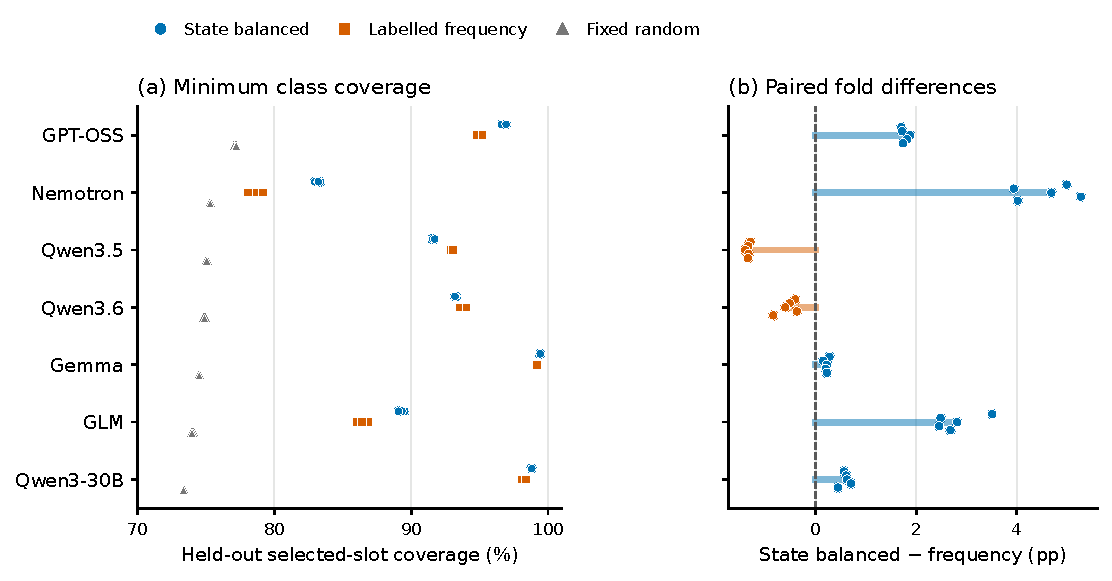
\includegraphics[width=\linewidth]{generated/best_results_20261009/heldout_retention.pdf}
\caption{Minimum held-out reasoning-class coverage at 75\% expert retention.
(a) All five common duplicate-family folds for each selection method;
horizontal lines connect the fold extrema. (b) All five paired
state-balanced-minus-frequency differences; bars end at their descriptive
fold mean. Coverage averages layers within class before taking the minimum.
The comparison uses training-only selection and identical quotas. Neither
fold ranges nor mean bars are inferential intervals.}
\label{fig:expert-memory-heldout}
\end{figure}

The comparison shows that balancing labelled states can improve the
least-covered class at a fixed identity budget, but the direction and
magnitude depend on the model. Near-complete coverage in Gemma and
Qwen3-30B also leaves little room for a large coverage improvement.
These observations establish neither accuracy retention after physical
removal nor a realized GPU-memory saving. Missing and unlabelled tokens
remain outside this class-conditioned endpoint.


\section{Interventions and Deployment Limits}

Historical sparse interventions demonstrate that candidate experts can
be engaged: pair-target inclusion changes by $+0.1376$
$[0.0763,0.1882]$ across eight families in study A and $+0.2940$
$[0.1277,0.4761]$ across thirteen in study B. This verifies an effect on
routing. The larger FRESH verification comparison estimates a semantic
success change of $+5.5$ percentage points against native, with
simultaneous 95\% interval $[-4.5,+15.5]$. Missing semantic judgments widen
the identification range. The retained global-steering comparisons also
show that some routing policies can substantially reduce accuracy; all
reported policies and their uncertainty remain in the appendix.

For a user deciding whether to deactivate experts or constrain routes,
usefulness is a paired change in answer quality and resource use on
independent evaluation families. A nonsignificant accuracy difference
does not establish retention. Such a claim needs a prespecified acceptable
loss margin and an interval precise enough to assess it. Expert exclusion
also needs matched random exclusions with comparable exposure, and actual
measurement of the claimed deployment saving. Actual expert-memory reduction requires omitted expert weights to be
absent from the measured resident model. Masking an expert while retaining
its weights is an intervention test, not evidence of a smaller memory
footprint. The reported deployment objective must therefore pair memory
measurements with accuracy and account for shared experts and the
unchanged dense parameters. Such a reduced-memory deployment has not yet
been measured here.

The separate verification study passed all 14 engineering checks for all
seven checkpoints. Its source-bound observation snapshot reports
model-specific recognition and control gates in
Table~\ref{tab:verification-status}. A model that
fails its full frozen recognition qualification stops before target
nomination and treatment under that controller; its causal and utility
cells remain unmeasured. These are limits of this controller and measurement
pipeline, not evidence that all routing interventions fail. Every checkpoint
retains its own gates; the full observed audits and the separate answer-grader
limit are reported in Appendix~\ref{sec:verification-study}.

\section{Discussion}

Routing supplies additional information about automatically labelled
reasoning episodes in all seven models under the declared text controls.
The next-class results refine this finding for two checkpoints, where
past routing adds to past text and history. Their effect sizes depend on
the generated text, annotation coverage and prediction task. They neither
establish latent cognitive modules nor identify a universal controller.

The held-out selection comparison supplies a further distinction:
reasoning-class balance is useful for coverage in some architectures and
less useful than labelled frequency in others. The common five-fold
comparison makes that model dependence visible without using correctness
to rank experts. Its endpoint is coverage of original selected slots;
post-removal generation can change the routes and subsequent text.
Thus even near-complete native coverage cannot establish preserved answer
accuracy or realized memory savings.

Labels are measurements of visible text, with imperfect annotation and
sparse coverage. Families define independent problem units, while saved
uncertainty remains conditional on the original fits and selections.
Exploratory same-cohort expert/correctness correlations and descriptive
concentration curves are preserved in Appendix~\ref{sec:saved-data-supplement}
with their original limitations. They do not select the main reported
results or justify suppressing a class-associated expert. Historical
intervention uncertainty, harmful policies and failed qualification gates
also remain visible in the appendices.

The present evidence supports routing readout and model-dependent
selection coverage. A deployment claim needs a separate controlled
measurement of answer quality and resident memory after actual removal,
including random and relevant pruning controls. That joint outcome
remains unestablished for the seven-model comparison.
